% Options for packages loaded elsewhere
\PassOptionsToPackage{unicode}{hyperref}
\PassOptionsToPackage{hyphens}{url}
%
\documentclass[
]{article}
\usepackage{lmodern}
\usepackage{amssymb,amsmath}
\usepackage{ifxetex,ifluatex}
\ifnum 0\ifxetex 1\fi\ifluatex 1\fi=0 % if pdftex
  \usepackage[T1]{fontenc}
  \usepackage[utf8]{inputenc}
  \usepackage{textcomp} % provide euro and other symbols
\else % if luatex or xetex
  \usepackage{unicode-math}
  \defaultfontfeatures{Scale=MatchLowercase}
  \defaultfontfeatures[\rmfamily]{Ligatures=TeX,Scale=1}
\fi
% Use upquote if available, for straight quotes in verbatim environments
\IfFileExists{upquote.sty}{\usepackage{upquote}}{}
\IfFileExists{microtype.sty}{% use microtype if available
  \usepackage[]{microtype}
  \UseMicrotypeSet[protrusion]{basicmath} % disable protrusion for tt fonts
}{}
\makeatletter
\@ifundefined{KOMAClassName}{% if non-KOMA class
  \IfFileExists{parskip.sty}{%
    \usepackage{parskip}
  }{% else
    \setlength{\parindent}{0pt}
    \setlength{\parskip}{6pt plus 2pt minus 1pt}}
}{% if KOMA class
  \KOMAoptions{parskip=half}}
\makeatother
\usepackage{xcolor}
\IfFileExists{xurl.sty}{\usepackage{xurl}}{} % add URL line breaks if available
\IfFileExists{bookmark.sty}{\usepackage{bookmark}}{\usepackage{hyperref}}
\hypersetup{
  hidelinks,
  pdfcreator={LaTeX via pandoc}}
\urlstyle{same} % disable monospaced font for URLs
\usepackage[margin=1in]{geometry}
\usepackage{graphicx,grffile}
\makeatletter
\def\maxwidth{\ifdim\Gin@nat@width>\linewidth\linewidth\else\Gin@nat@width\fi}
\def\maxheight{\ifdim\Gin@nat@height>\textheight\textheight\else\Gin@nat@height\fi}
\makeatother
% Scale images if necessary, so that they will not overflow the page
% margins by default, and it is still possible to overwrite the defaults
% using explicit options in \includegraphics[width, height, ...]{}
\setkeys{Gin}{width=\maxwidth,height=\maxheight,keepaspectratio}
% Set default figure placement to htbp
\makeatletter
\def\fps@figure{htbp}
\makeatother
\setlength{\emergencystretch}{3em} % prevent overfull lines
\providecommand{\tightlist}{%
  \setlength{\itemsep}{0pt}\setlength{\parskip}{0pt}}
\setcounter{secnumdepth}{-\maxdimen} % remove section numbering
\usepackage[USenglish]{babel}
\usepackage{fancyhdr}
\pagestyle{fancy}
\renewcommand{\sectionmark}[1]{\markright{#1}}
\fancyhf{}
\lhead{{}}
\rhead{{\today}}
\cfoot{{\thepage}}
\usepackage[T1]{fontenc}
\usepackage{bm}
\usepackage{mathpazo}
\usepackage{lscape}
\usepackage{pdfpages}
\newcommand{\blandscape}{\begin{landscape}}
\newcommand{\elandscape}{\end{landscape}}
\usepackage{tabularx}
\usepackage{titlesec}
\usepackage{graphicx,xcolor}
\usepackage{wrapfig}
\usepackage{amssymb}
\usepackage{amsmath}
\usepackage{esint}
\usepackage{paralist}
\usepackage{outlines}
\newcommand{\I}{\textrm{I}}
\newcommand{\N}{\mathcal{N}}
\newcommand{\D}{\textrm{D}}
\newcommand{\E}{\mathbb{E}}
\setlength{\parskip}{1em}%0.5\baselineskip
\setlength{\parindent}{0pt}
\linespread{1.15}
\titleformat*{\section}{\Large\scshape\bfseries}
\titleformat*{\subsection}{\large\scshape\bfseries}
\titleformat*{\subsubsection}{\bfseries}
\titleformat*{\paragraph}{\bfseries}
\titleformat*{\subparagraph}{\bfseries}
\renewcommand{\thesection}{\Roman{section}.}%1.A.assubsections
\renewcommand{\thesubsection}{\Alph{subsection}.}%1.A.assubsections
\titlespacing{\section}{0pt}{2pt}{3pt}
\titlespacing{\subsection}{0pt}{2pt}{2pt}
\titlespacing{\subsubsection}{0pt}{0pt}{0pt}
\titlespacing{\paragraph}{0pt}{1pt}{5pt}
\titlespacing{\subparagraph}{10pt}{1pt}{5pt}
\usepackage{hyperref}
\usepackage[font={footnotesize}]{subcaption}
\usepackage[font={footnotesize}]{caption}
\usepackage{caption,setspace}
\captionsetup{font={stretch=1}}
\captionsetup[figure]{font=footnotesize,labelfont=footnotesize}
\usepackage{tabto}
\def\quoteattr#1#2{\setbox0=\hbox{#2}#1\tabto{\dimexpr\linewidth-\wd0}\box0}
\makeatletter
\newcommand{\pushright}[1]{\ifmeasuring@#1\hfill$\displaystyle#1$\fi\ignorespaces}
\makeatother
\newcommand{\FixMe}[1]{\textcolor{orange}{[#1]}}
\newcommand{\Comment}[1]{\textcolor{purple}{\textit{[#1]}}}
\newcommand{\Quickwin}{{\color{blue}{$\bigstar$}}}
\usepackage{letltxmacro}
\LetLtxMacro\Oldfootnote\footnote
\newcommand{\EnableFootNotes}{\LetLtxMacro\footnote\Oldfootnote}
\newcommand{\DisableFootNotes}{\renewcommand{\footnote}[2][]{\relax}}
\makeatother
\graphicspath{{../Output/"}}
\renewcommand{\thefigure}{S\arabic{figure}}
% Bibliography
\usepackage{natbib}
\bibliographystyle{aer}
\setcitestyle{authoryear, open={(},close={)}}

\author{}
\date{\vspace{-2.5em}}

\begin{document}

\begin{center} 
    \textbf{\scshape \LARGE Supplemental Information}\\  \vspace{2mm}
    {\large Passing the Test}\\ \vspace{2mm} 
    {\large Alyssa Bilinski \footnote{Contact: abilinski@g.harvard.edu},\footnote{Data and code are available on GitHub (\href{https://github.com/abilinski/BackToSchool2}{link}).} $\cdot$ Joshua A. Salomon $\cdot$ Andrea Ciaranello \newline John Giardina $\cdot$ Meagan C. Fitzpatrick} \\
\end{center}

\hypertarget{figures}{%
\section{Figures}\label{figures}}

\begin{figure}
\centering
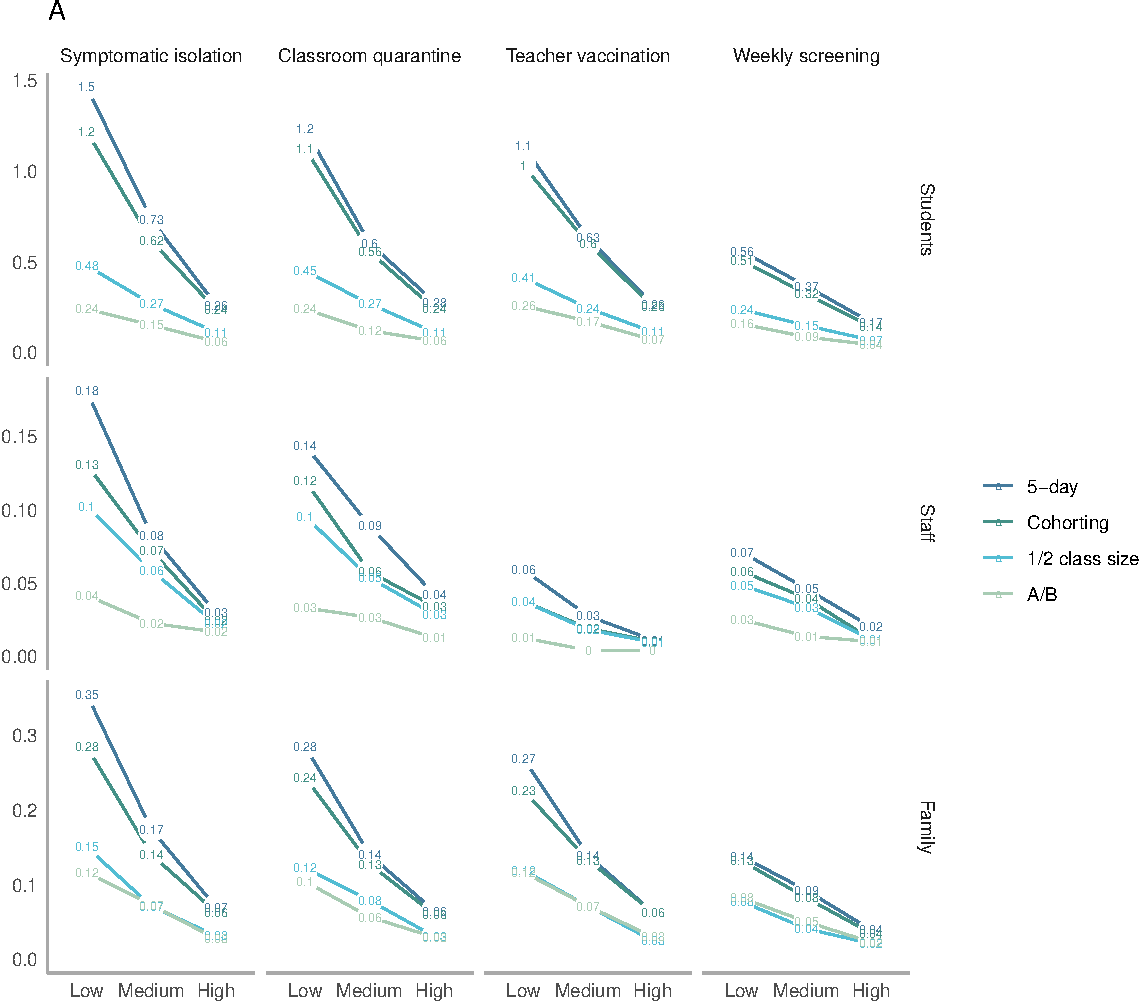
\includegraphics{Schools_supplement_files/figure-latex/figs1-1.pdf}
\caption{Sensitivity analysis - elementary schools by case type. Average
number of total secondary transmissions over 30 days (outside of the
index case's household) following a single introduction into an
elementary school community. These include both transmission directly
from the index case, as well as from secondary and tertiary cases. The
x-axes varies the level of prevention measure uptake, with low uptake
assuming minimal interventions and high uptake assuming intensive
interventions. Line colors correspond to scheduling strategies.}
\end{figure}

\begin{figure}
\centering
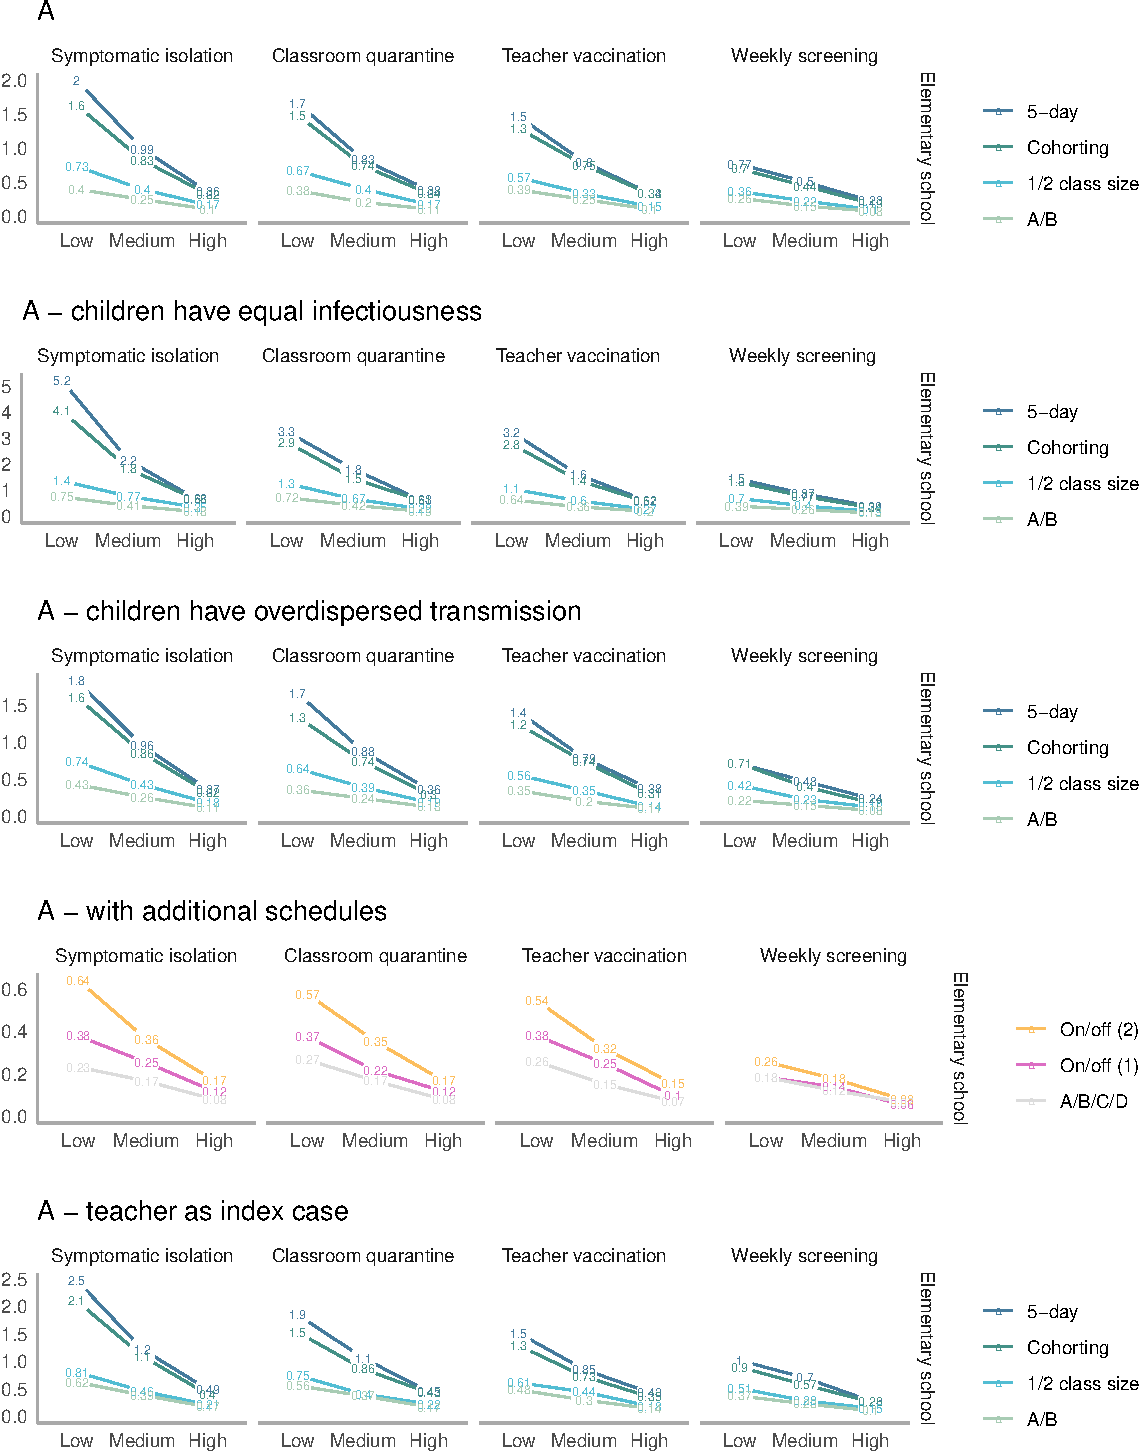
\includegraphics{Schools_supplement_files/figure-latex/figs3-1.pdf}
\caption{Sensitivity analyses (elementary schools) -- average number of
total secondary transmissions over 30 days (outside of the index case's
household) following a single introduction into a school community. The
columns vary the level of prevention measure uptake, with low uptake
assuming minimal interventions and high uptake assuming intensive
interventions. Line colors correspond to scheduling strategies.}
\end{figure}

\begin{figure}
\centering
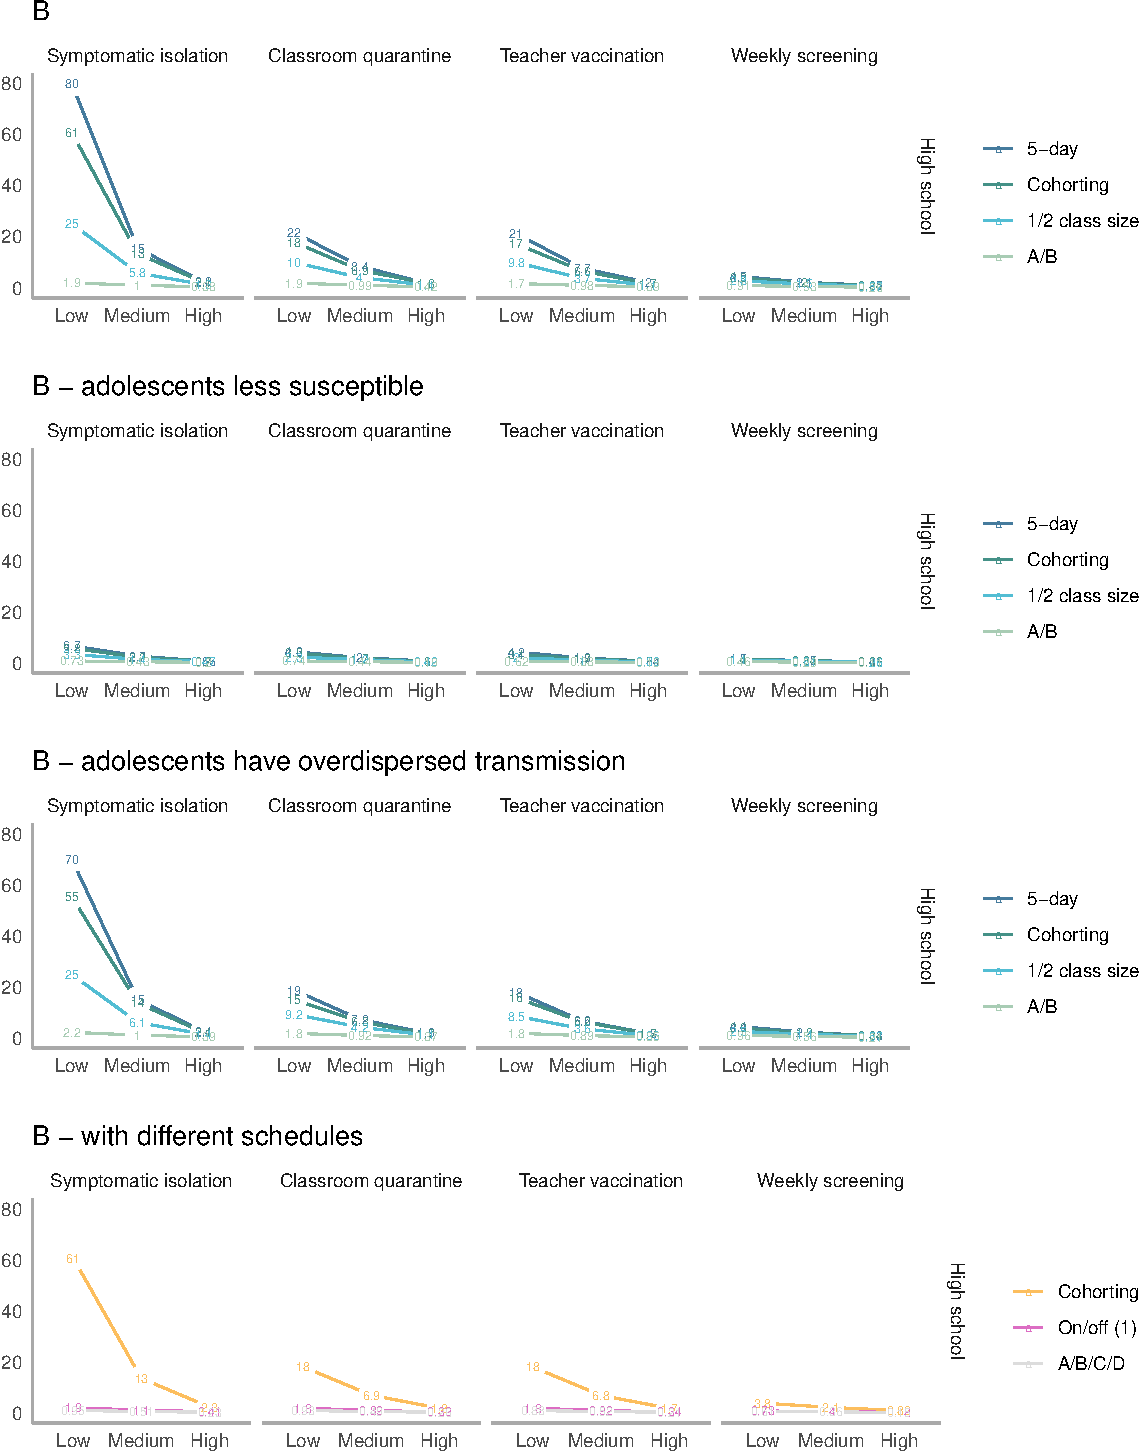
\includegraphics{Schools_supplement_files/figure-latex/figs4-1.pdf}
\caption{Sensitivity analyses (elementary schools) -- average number of
total secondary transmissions over 30 days (outside of the index case's
household) following a single introduction into a school community. The
columns vary the level of prevention measure uptake, with low uptake
assuming minimal interventions and high uptake assuming intensive
interventions. Line colors correspond to scheduling strategies.}
\end{figure}

\blandscape

\begin{figure}
\centering
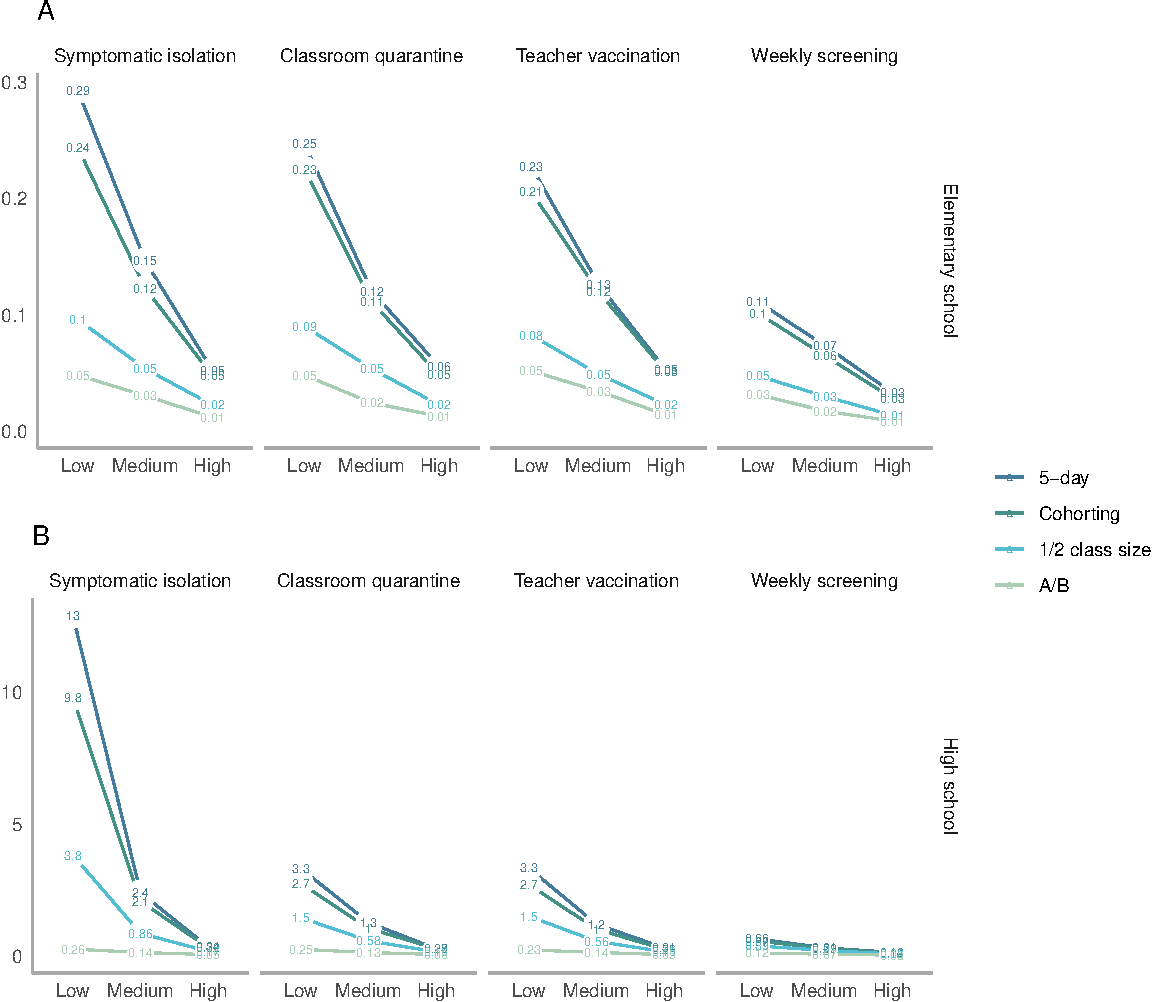
\includegraphics{Schools_supplement_files/figure-latex/fig2-1.pdf}
\caption{Average number of clinically symptomatic cases in staff and
students over 30 days following a single introduction into a school
community. These include both transmission directly from the index case,
as well as from secondary and tertiary cases. The top panel shows
elementary schools, where children are assumed to be less susceptible
and less infectious, while the bottom panel shows high schools. Note
that axes differ across rows. The x-axes varies the level of prevention
measure uptake, with low uptake assuming minimal interventions and high
uptake assuming intensive interventions. Line colors correspond to
scheduling strategies.}
\end{figure}

\elandscape

\begin{figure}
\centering
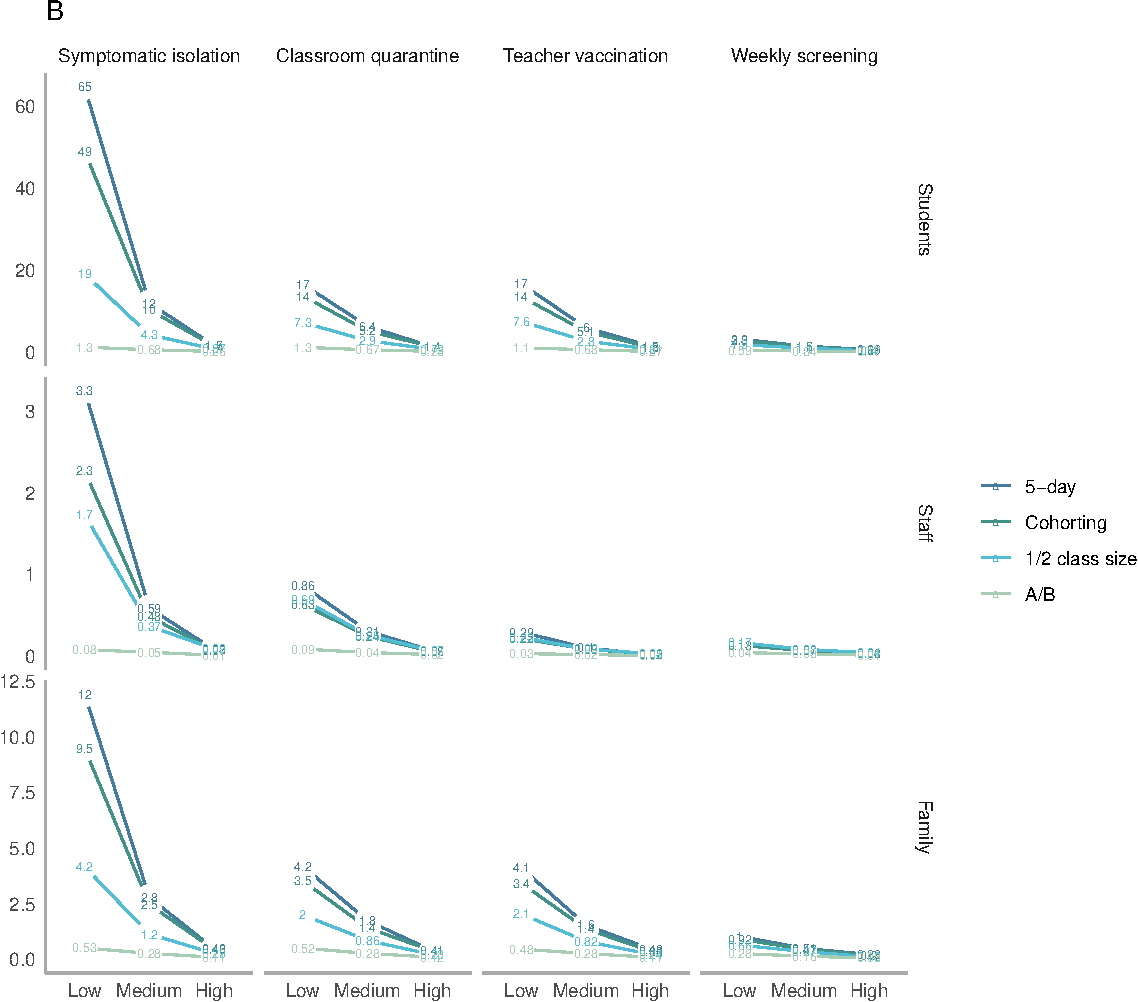
\includegraphics{Schools_supplement_files/figure-latex/figs2-1.pdf}
\caption{Sensitivity analysis - high schools by case type. Average
number of total secondary transmissions over 30 days (outside of the
index case's household) following a single introduction into an
elementary school community. These include both transmission directly
from the index case, as well as from secondary and tertiary cases. The
x-axes varies the level of prevention measure uptake, with low uptake
assuming minimal interventions and high uptake assuming intensive
interventions. Line colors correspond to scheduling strategies.}
\end{figure}

\blandscape

\begin{figure}
\centering
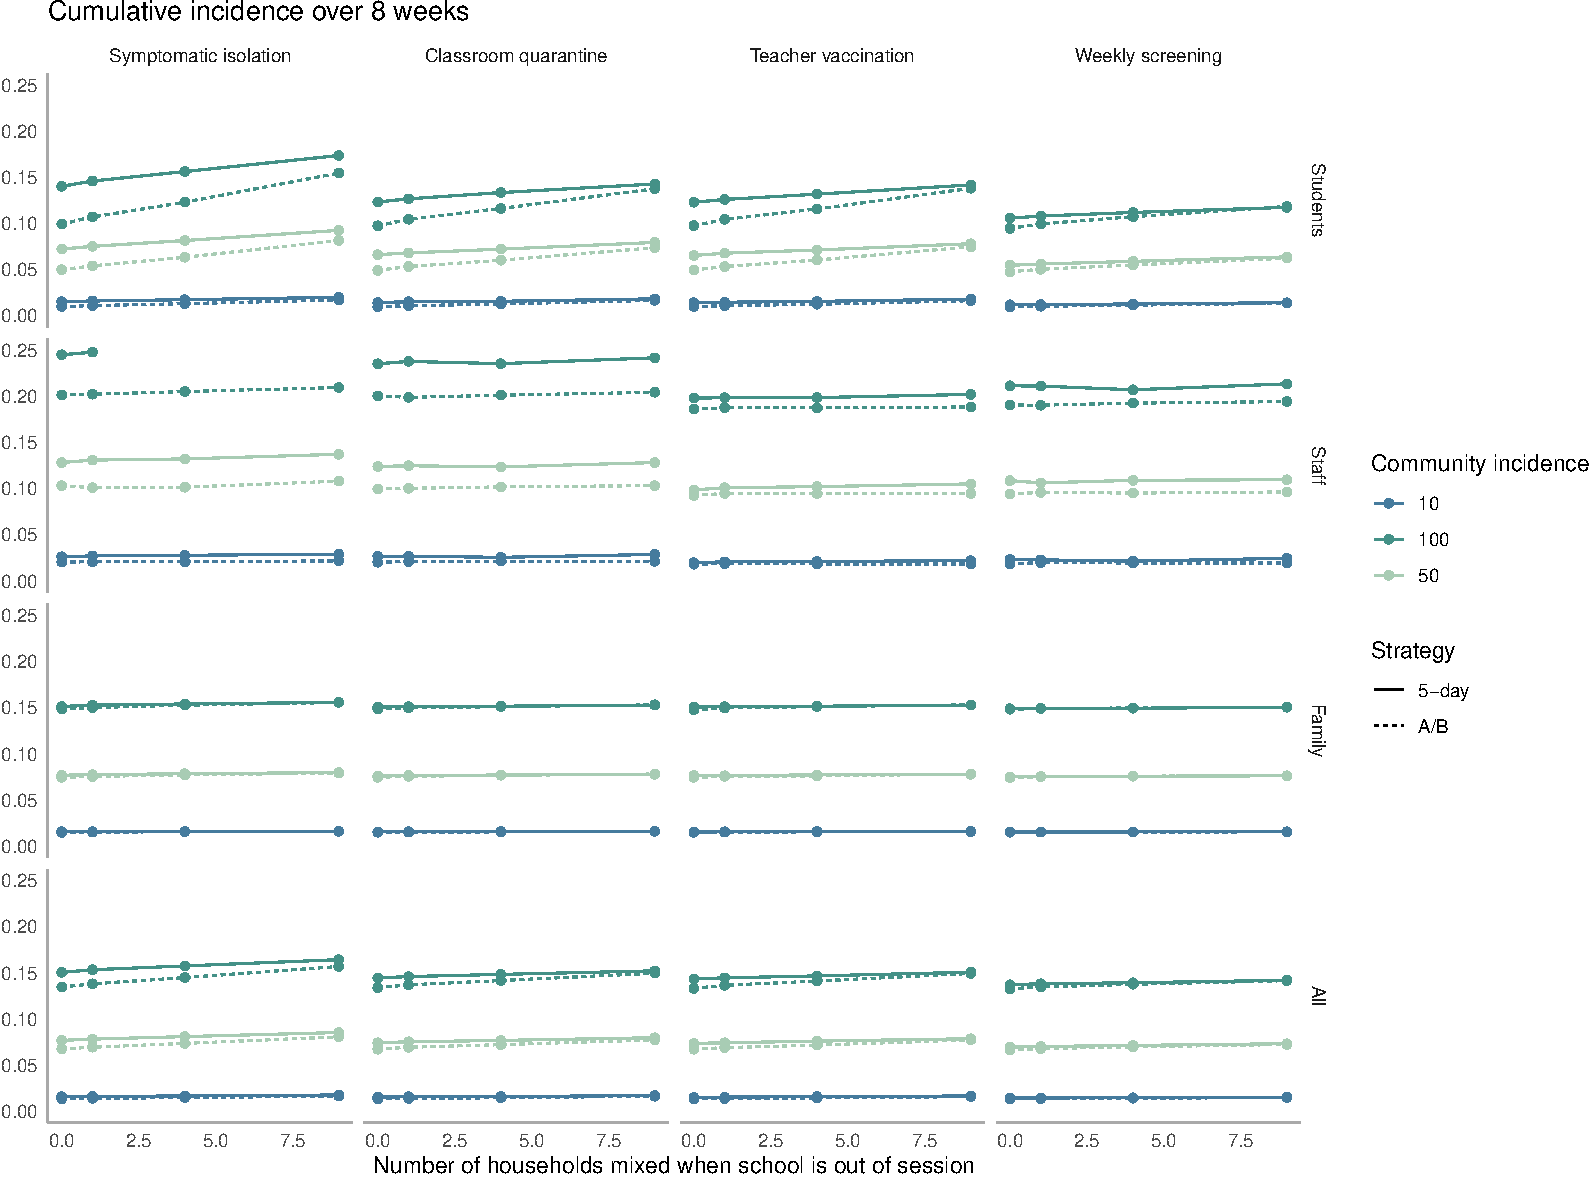
\includegraphics{Schools_supplement_files/figure-latex/unnamed-chunk-1-1.pdf}
\caption{Cumulative incidence over 8 weeks in elementary schools across
different levels of out-of-school mixing. The x-axis shows the average
daily community incidence per 100,000 population. The y-axis shows
cumulative incidence over 8 weeks. Columns denote different isolation,
quarantine, vaccination, and detection strategies, while rows show
different population subgroups.}
\end{figure}

\elandscape

\blandscape

\begin{figure}
\centering
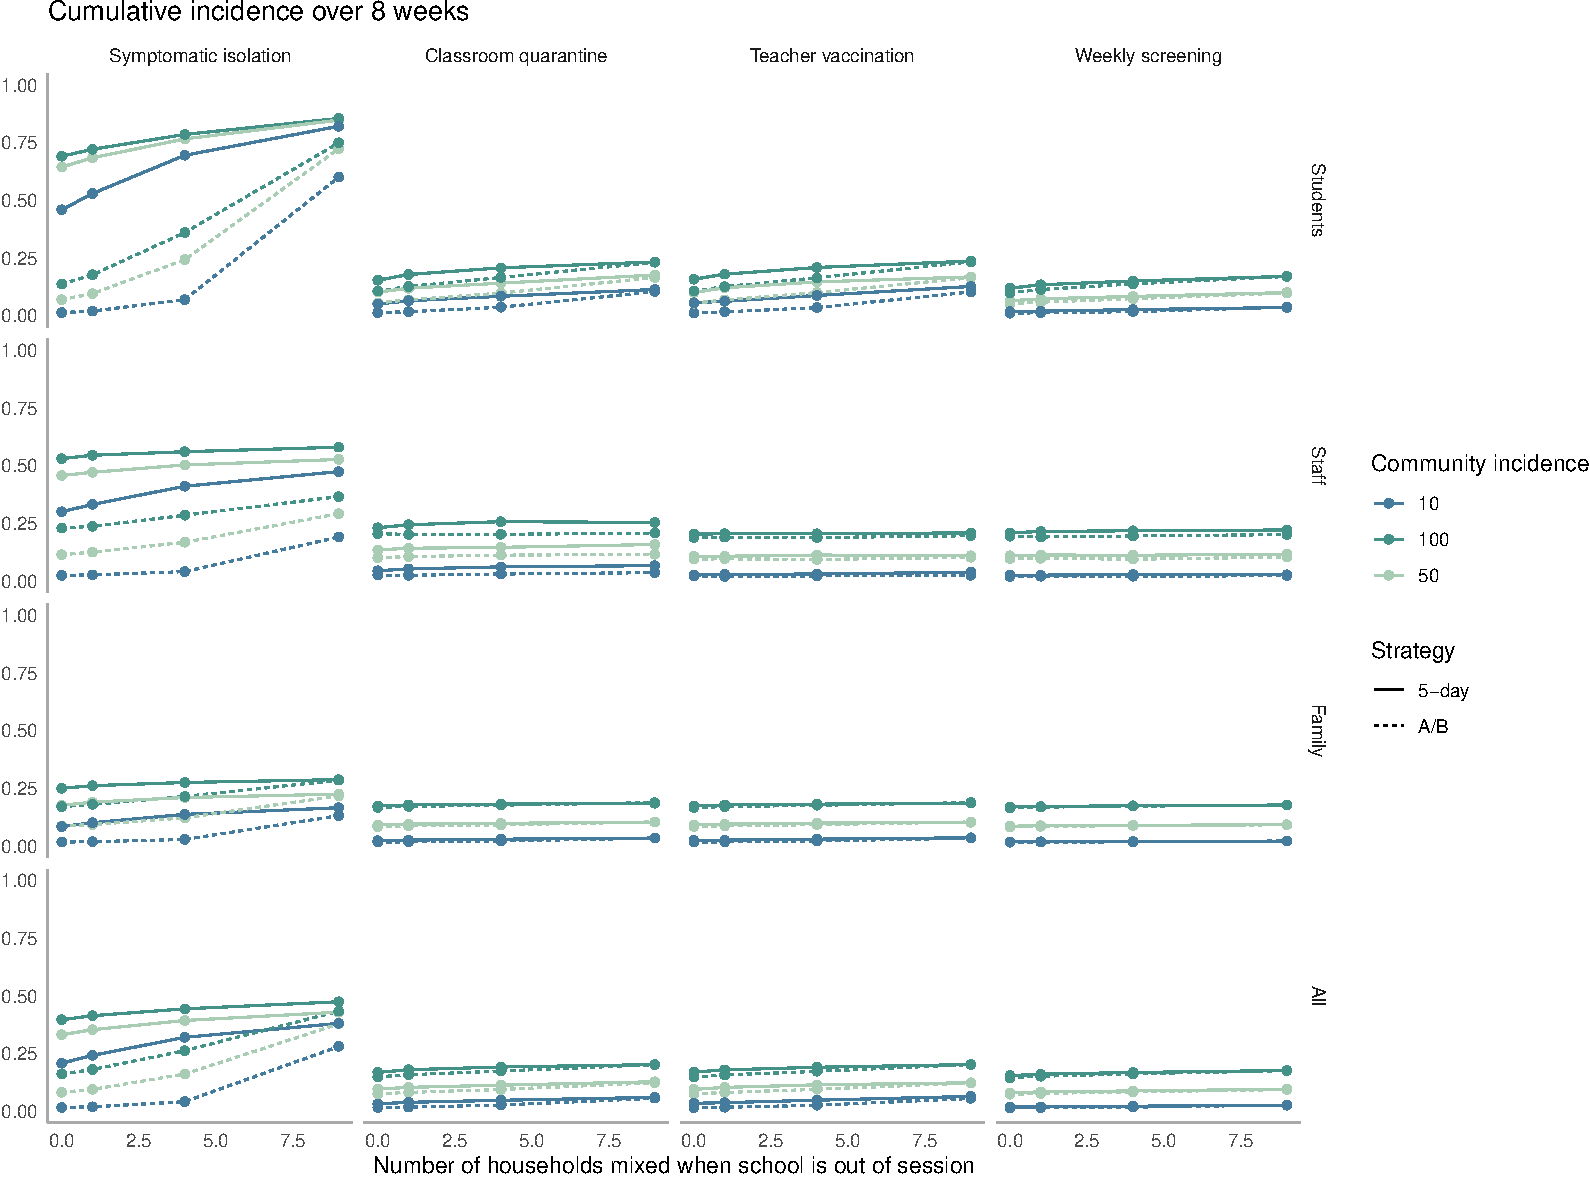
\includegraphics{Schools_supplement_files/figure-latex/unnamed-chunk-2-1.pdf}
\caption{Cumulative incidence over 8 weeks in high schools across
different levels of out-of-school mixing. The x-axis shows the average
daily community incidence per 100,000 population. The y-axis shows
cumulative incidence over 8 weeks. Columns denote different isolation,
quarantine, vaccination, and detection strategies, while rows show
different population subgroups.}
\end{figure}

\elandscape

\clearpage

\hypertarget{model}{%
\section{Model}\label{model}}

We use a Framework for Reconstructing Epidemiological Dynamics (FRED) to
generate household structures (Wheaton 2014). For computational
simplicity, we used Maryland as a representative state, as sibling
structure (the main parameter of interest) did not appear sensitive to
location.

\begin{tabular}{cccc}
Maryland Elementary & Connecticut Elementary & Mississippi Elementary  & Texas Elementary  \\
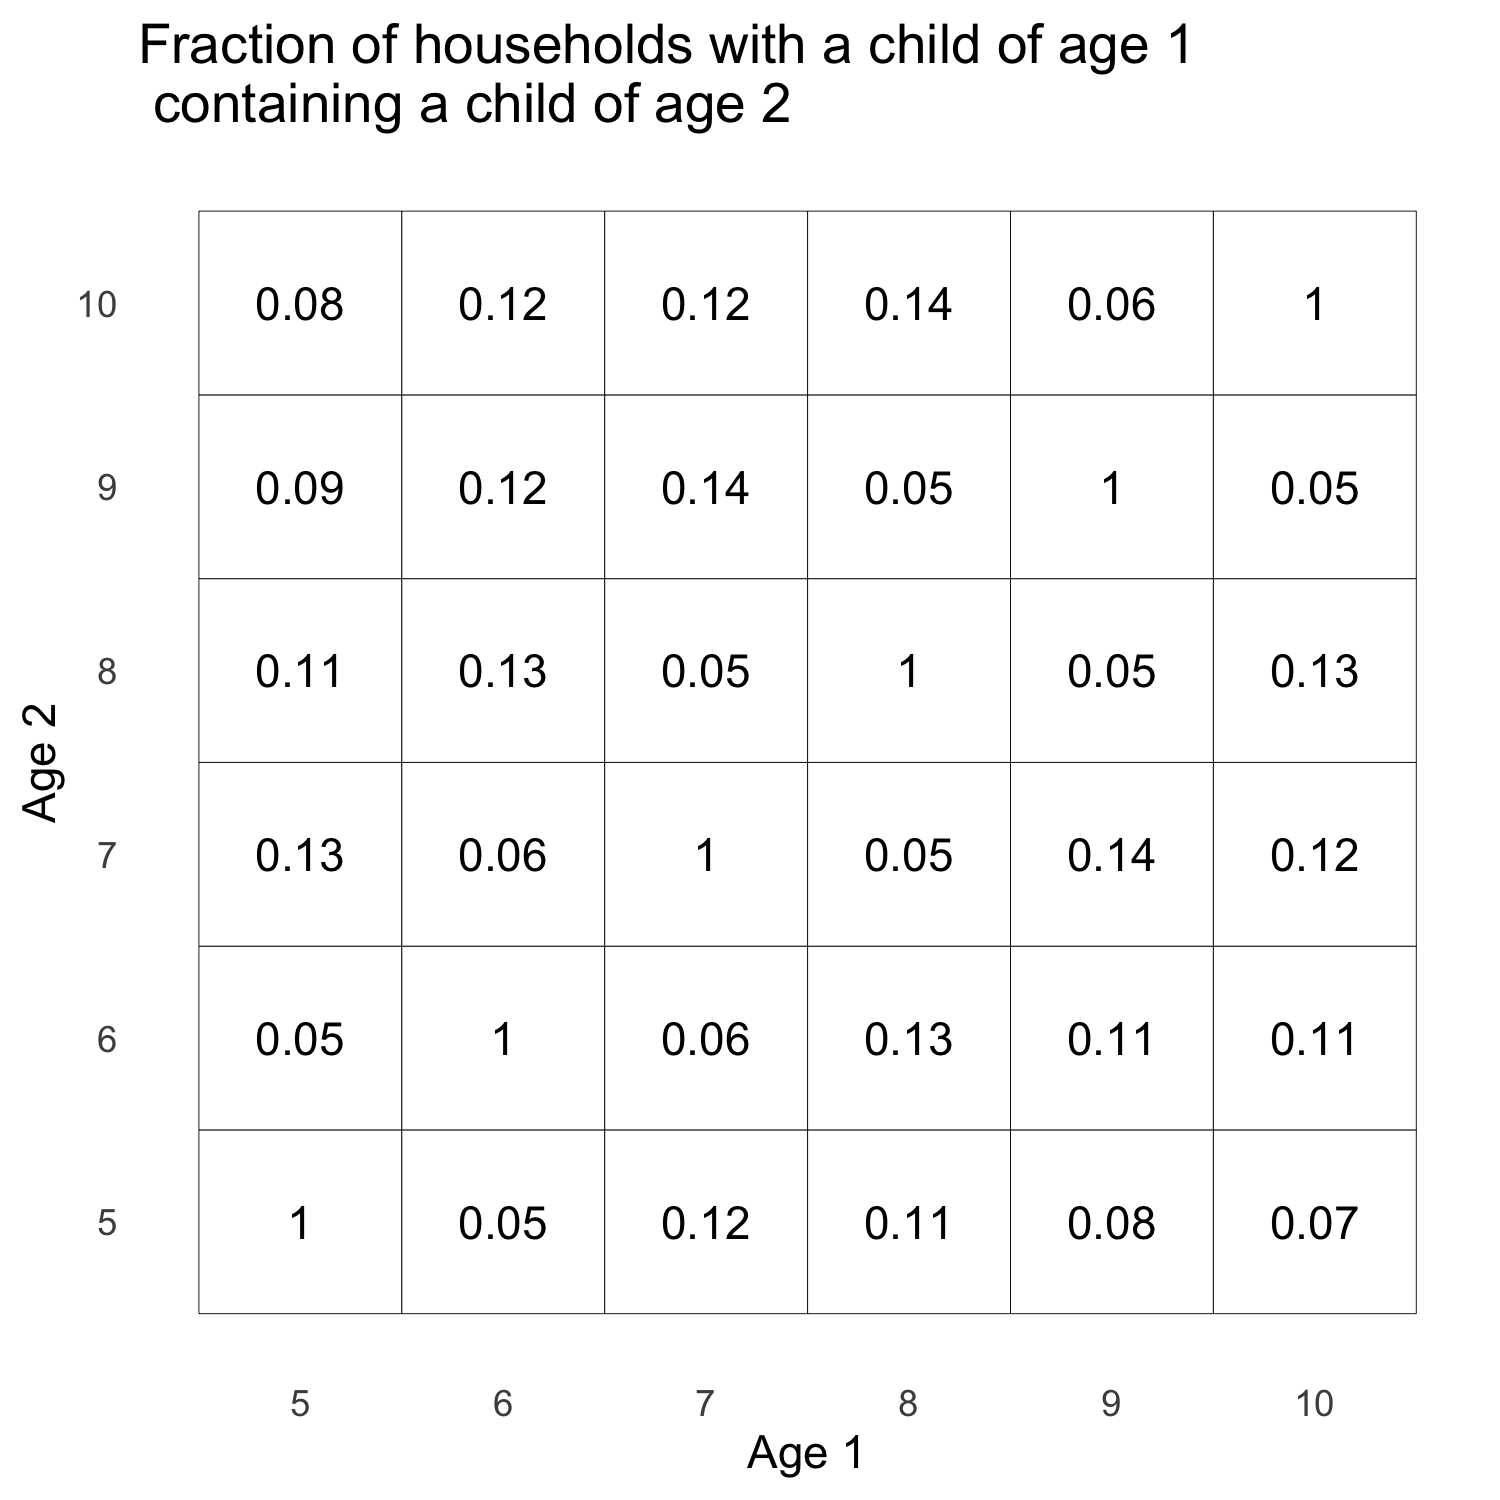
\includegraphics[width=40mm]{/Users/abilinski/Dropbox/Schools/Public code/0 - Synthetic Populations/2 - Output/sibling_heatmap_Maryland.png} &
      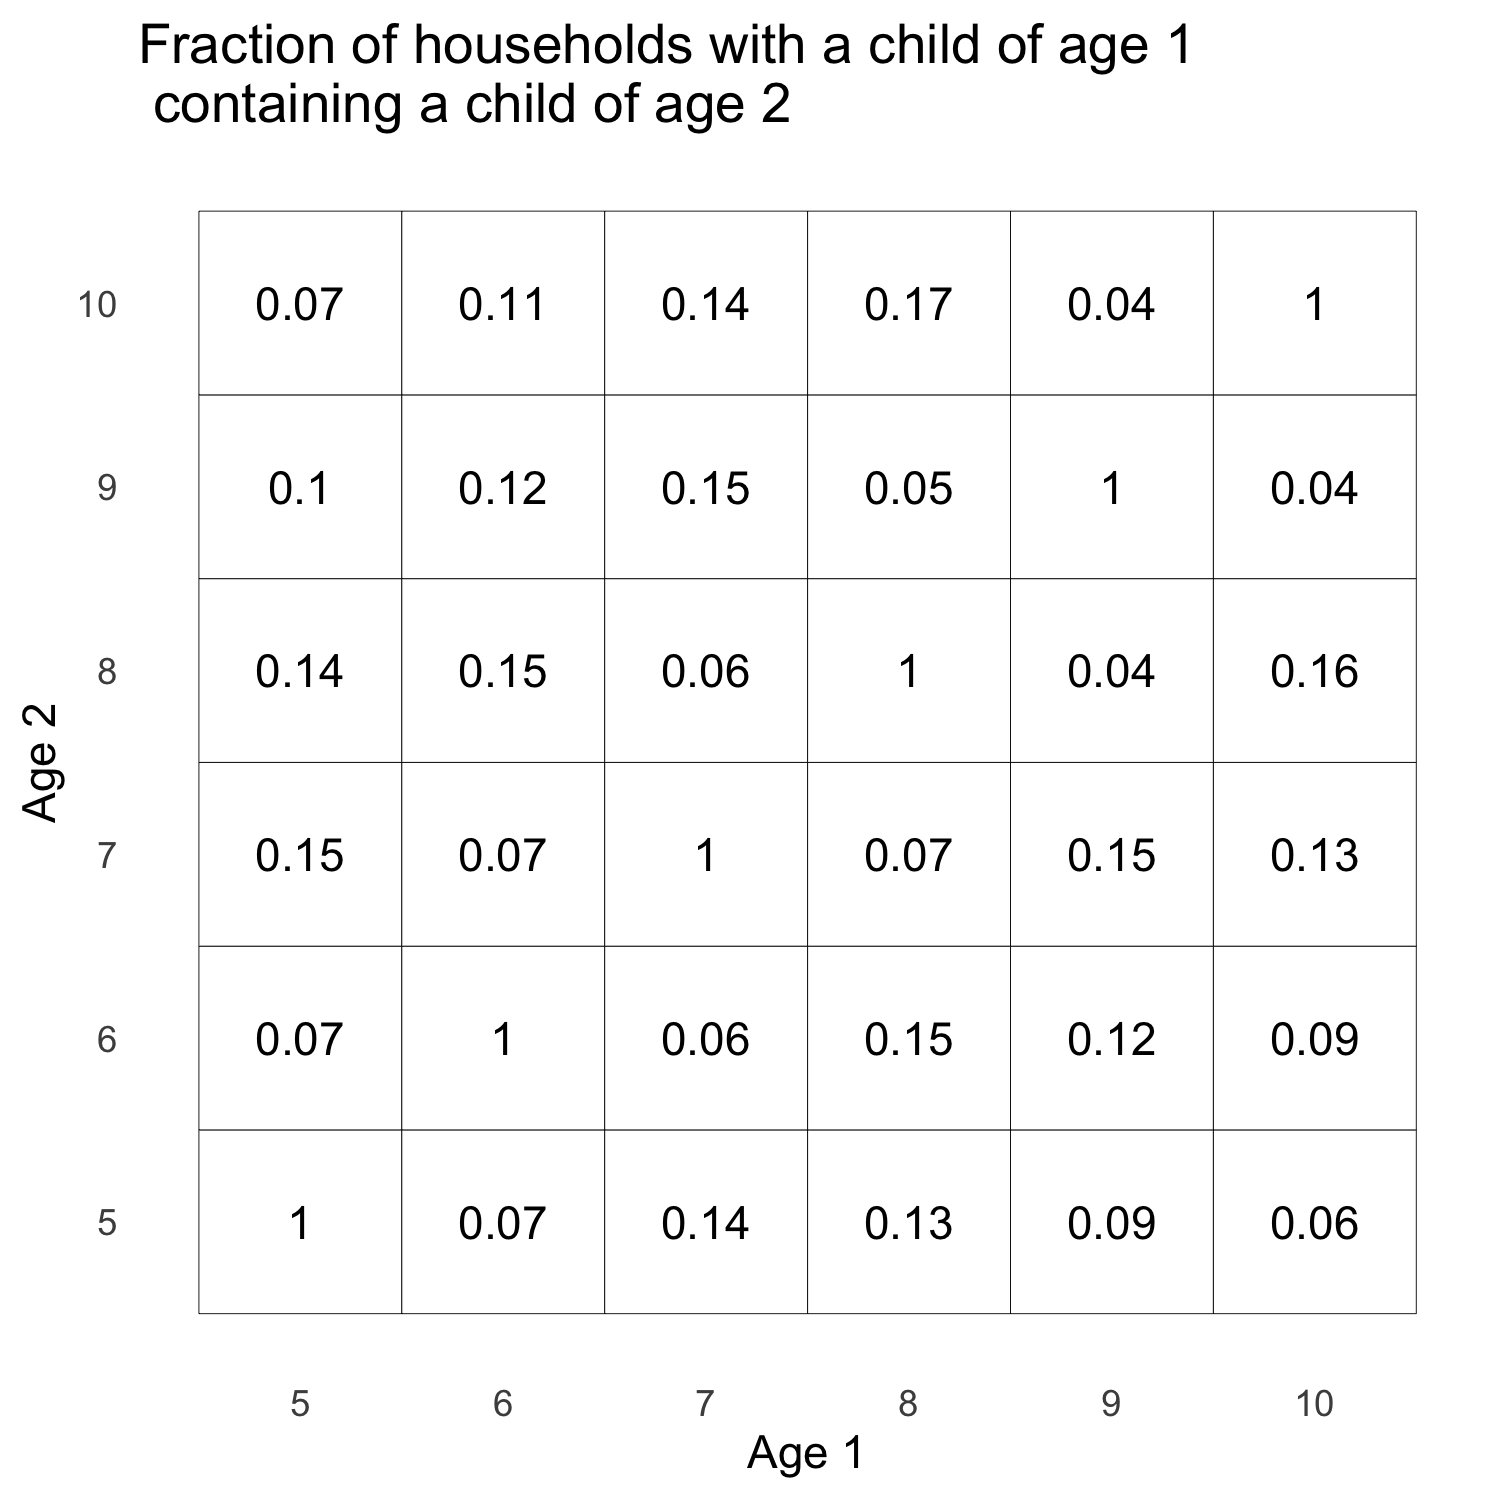
\includegraphics[width=40mm]{/Users/abilinski/Dropbox/Schools/Public code/0 - Synthetic Populations/2 - Output/sibling_heatmap_Connecticut.png} &
      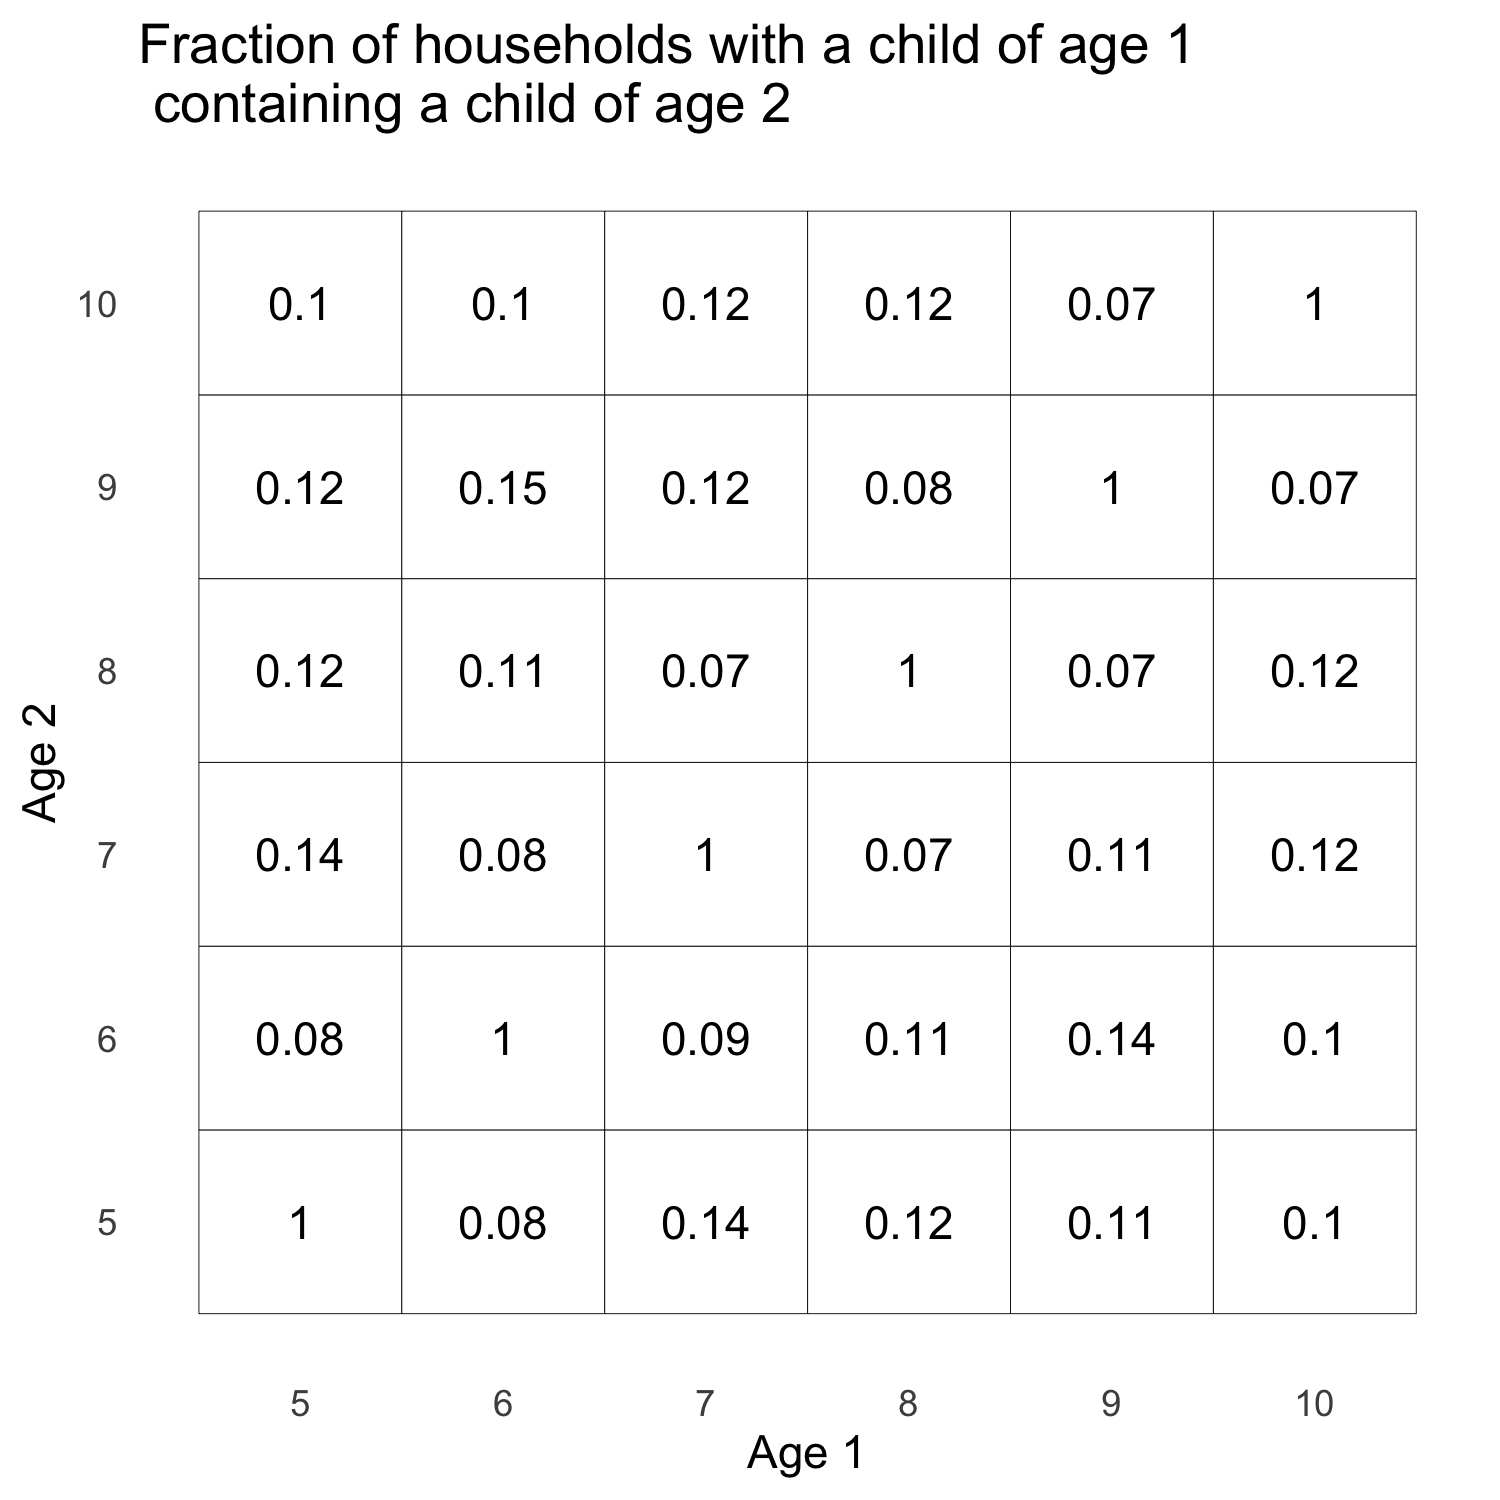
\includegraphics[width=40mm]{/Users/abilinski/Dropbox/Schools/Public code/0 - Synthetic Populations/2 - Output/sibling_heatmap_Mississippi.png} &
      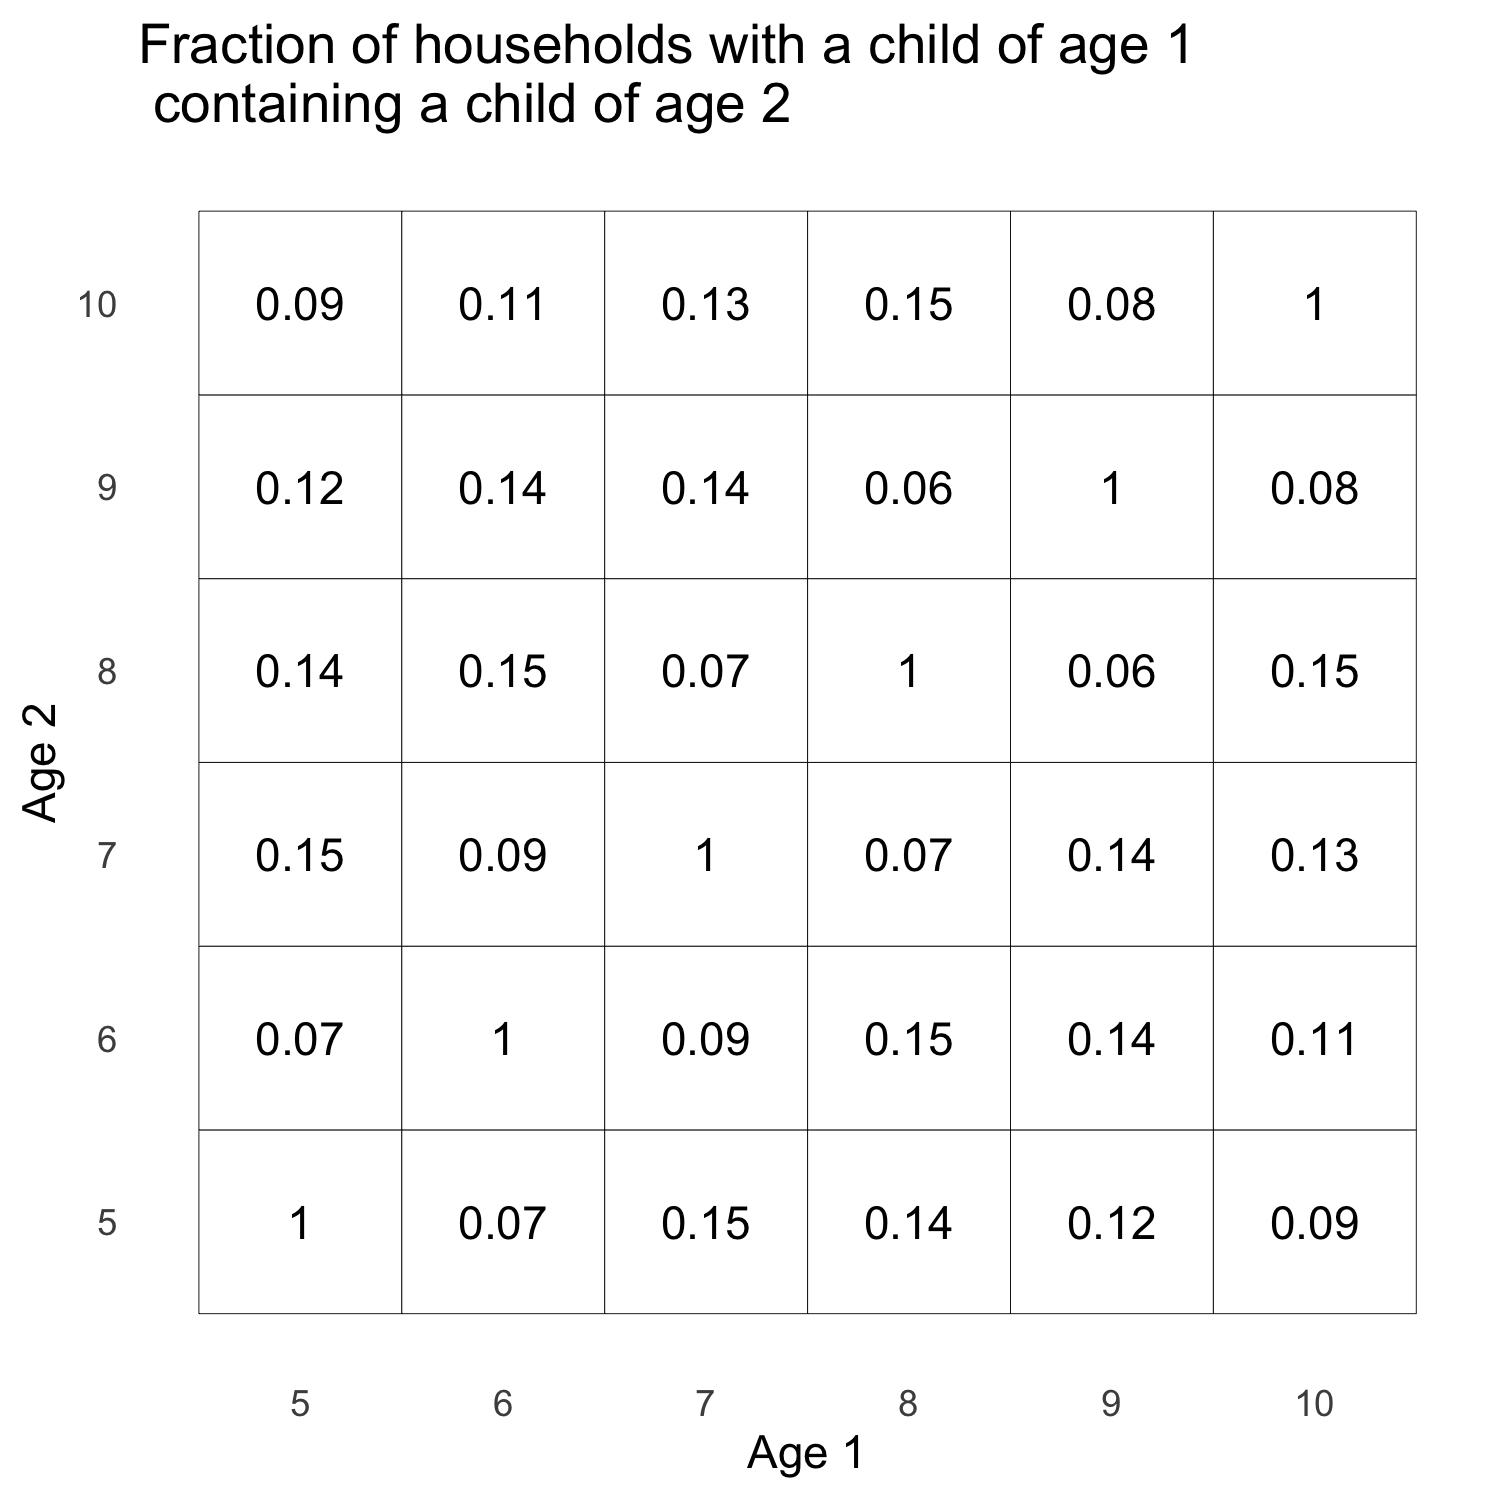
\includegraphics[width=40mm]{/Users/abilinski/Dropbox/Schools/Public code/0 - Synthetic Populations/2 - Output/sibling_heatmap_Texas.png} 
    \end{tabular}

\begin{tabular}{cccc}
Maryland HS & Connecticut HS & Mississippi HS  & Texas HS  \\
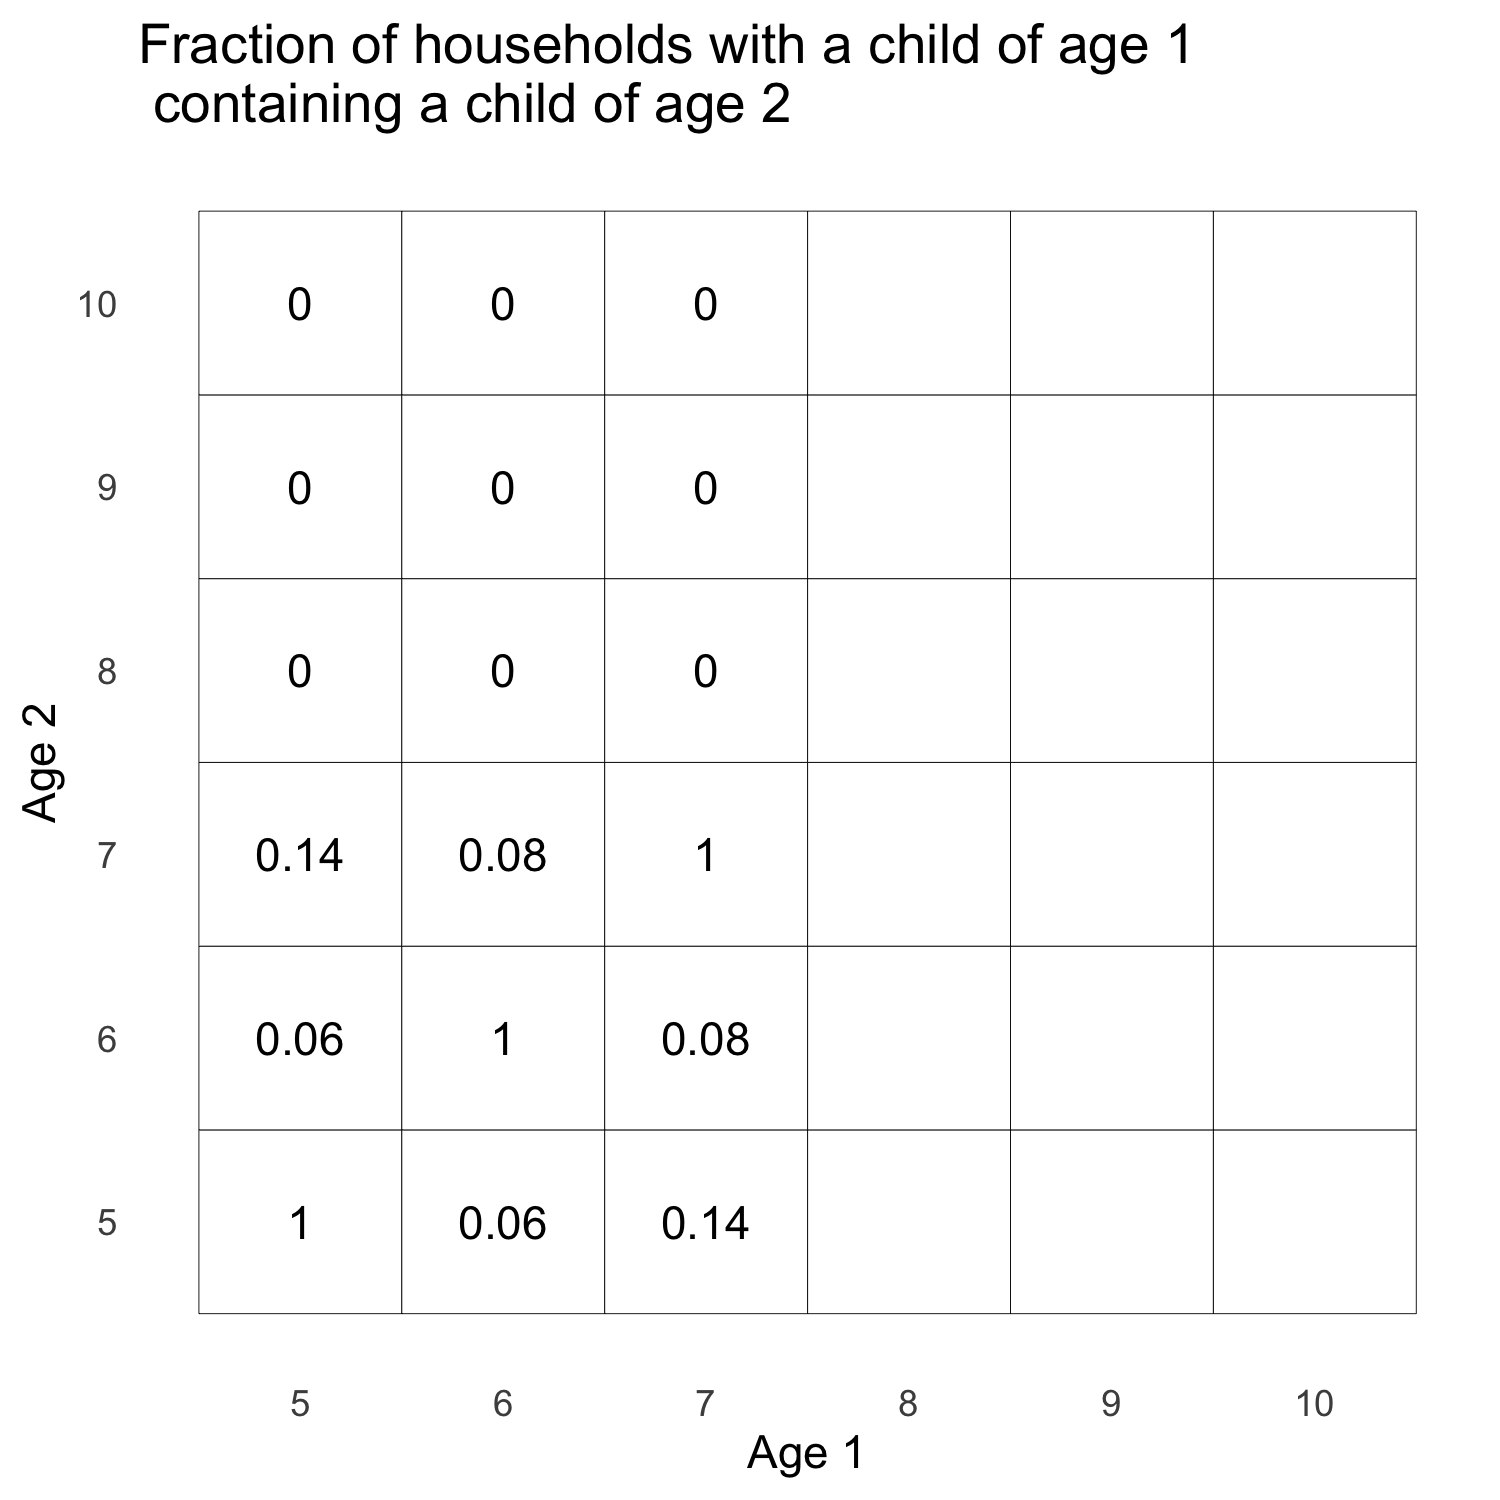
\includegraphics[width=40mm]{/Users/abilinski/Dropbox/Schools/Public code/0 - Synthetic Populations/2 - Output/sibling_heatmap_Maryland_HS.png} &
      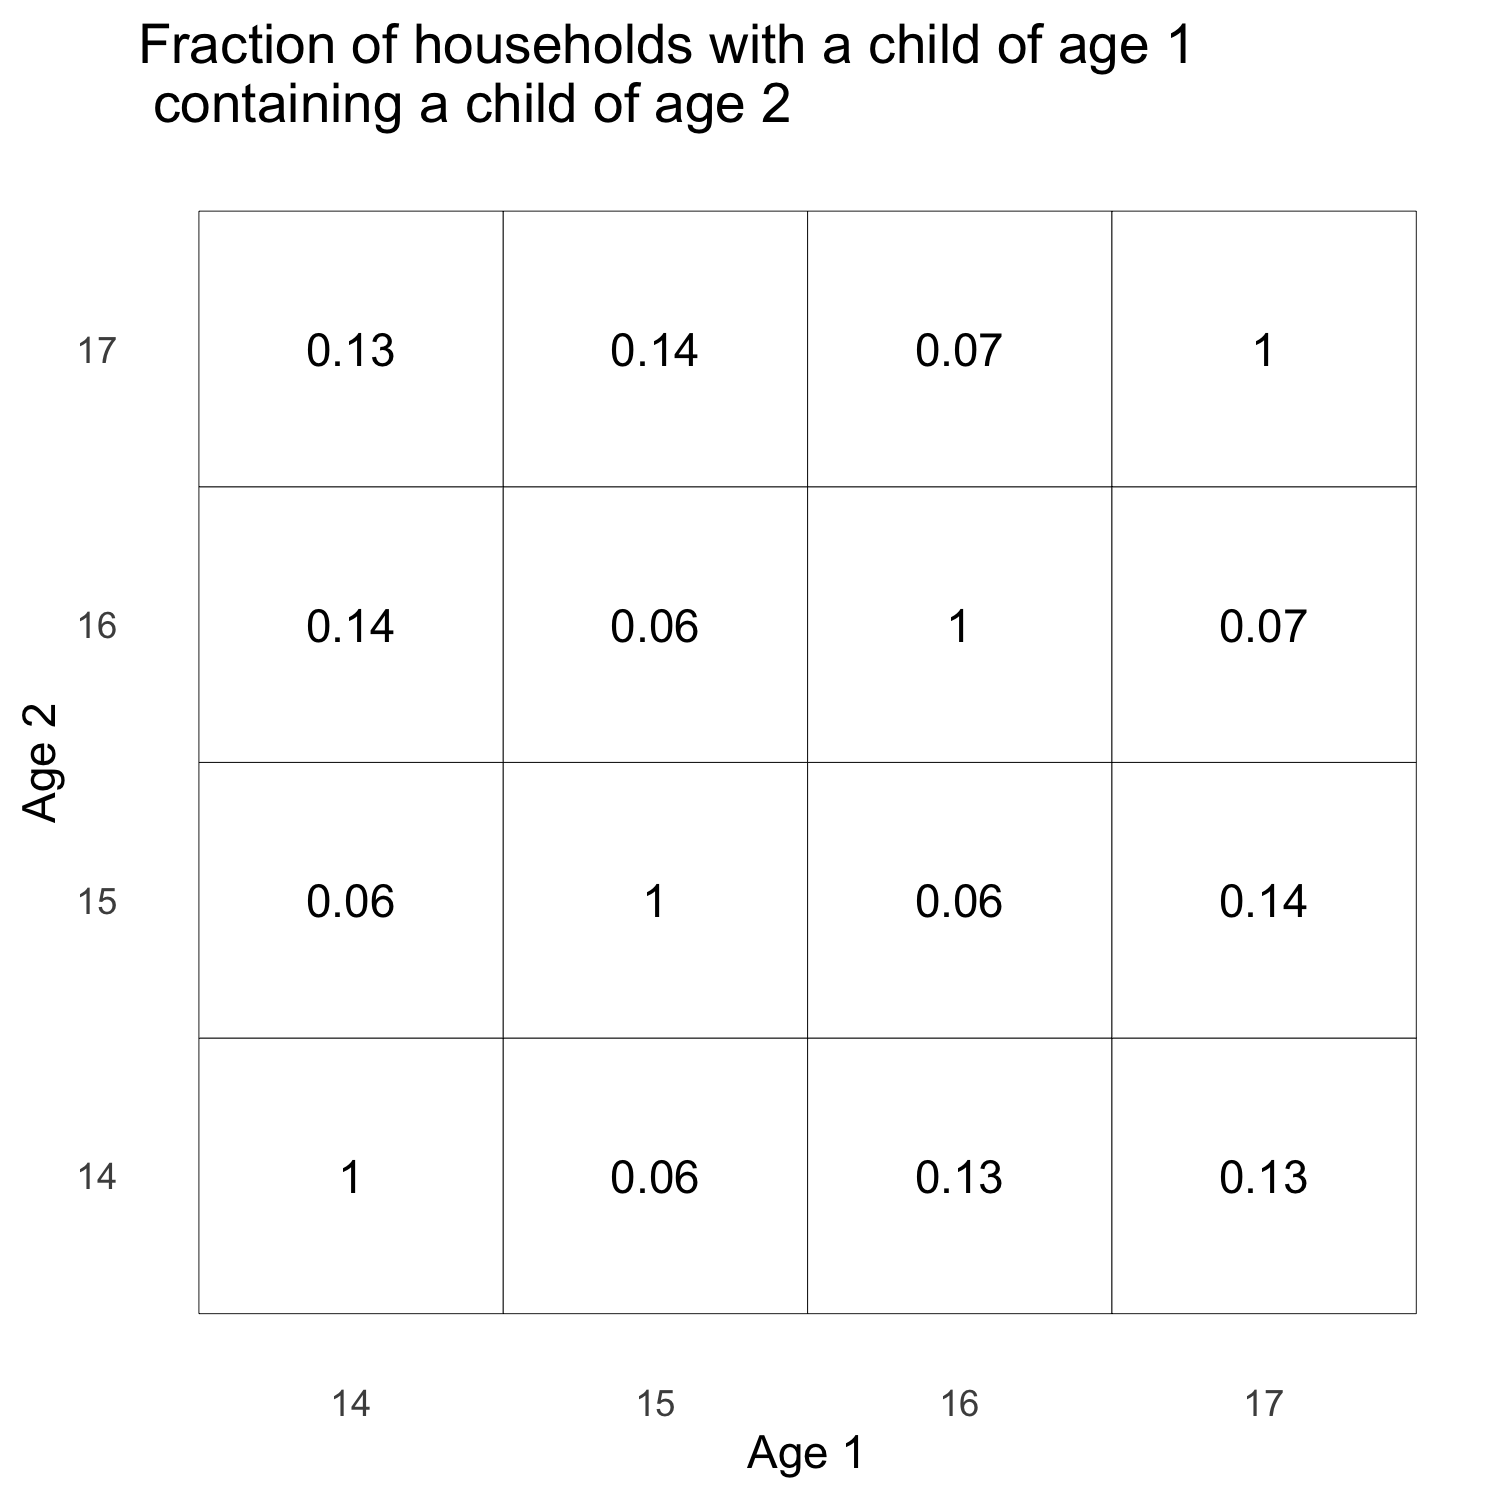
\includegraphics[width=40mm]{/Users/abilinski/Dropbox/Schools/Public code/0 - Synthetic Populations/2 - Output/sibling_heatmap_Connecticut_HS.png} &
      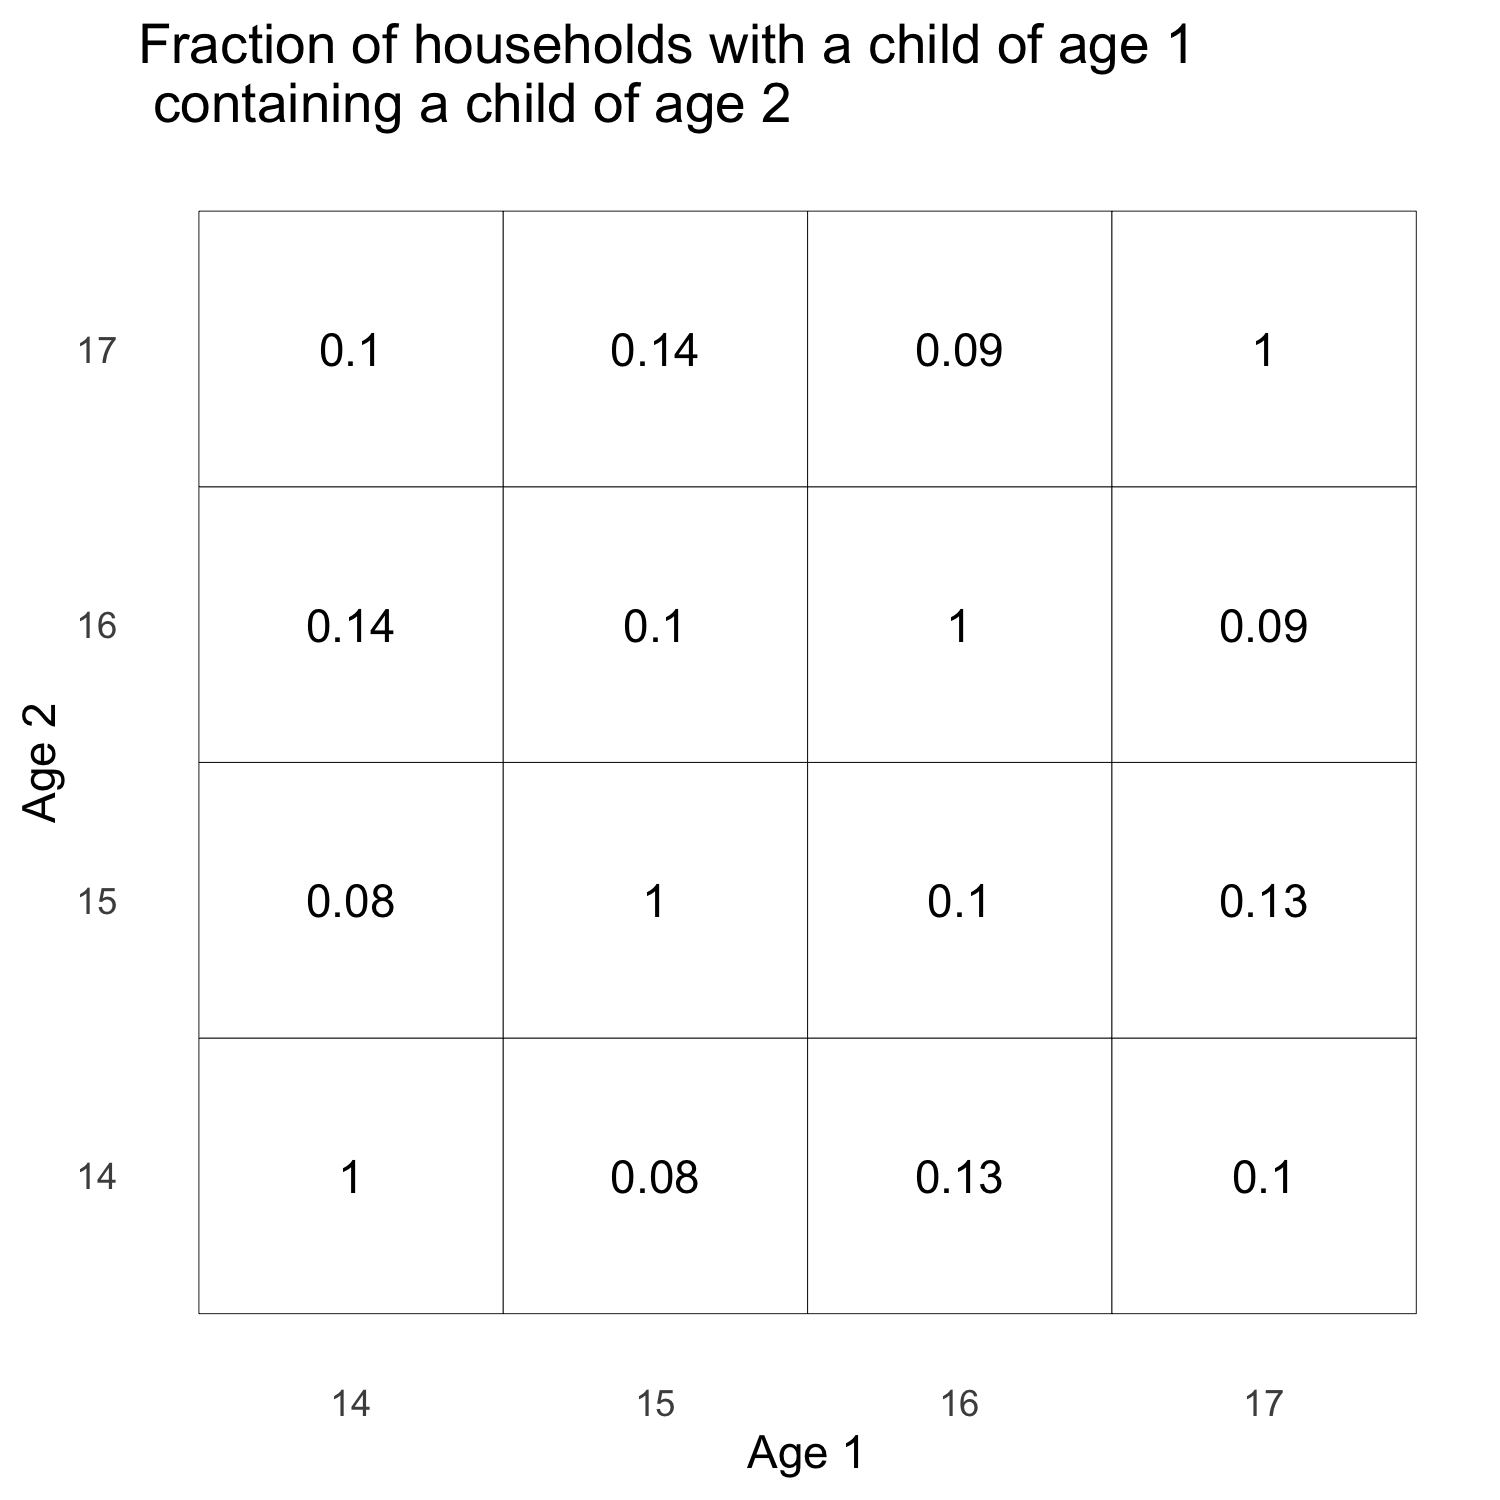
\includegraphics[width=40mm]{/Users/abilinski/Dropbox/Schools/Public code/0 - Synthetic Populations/2 - Output/sibling_heatmap_Mississippi_HS.png} &
      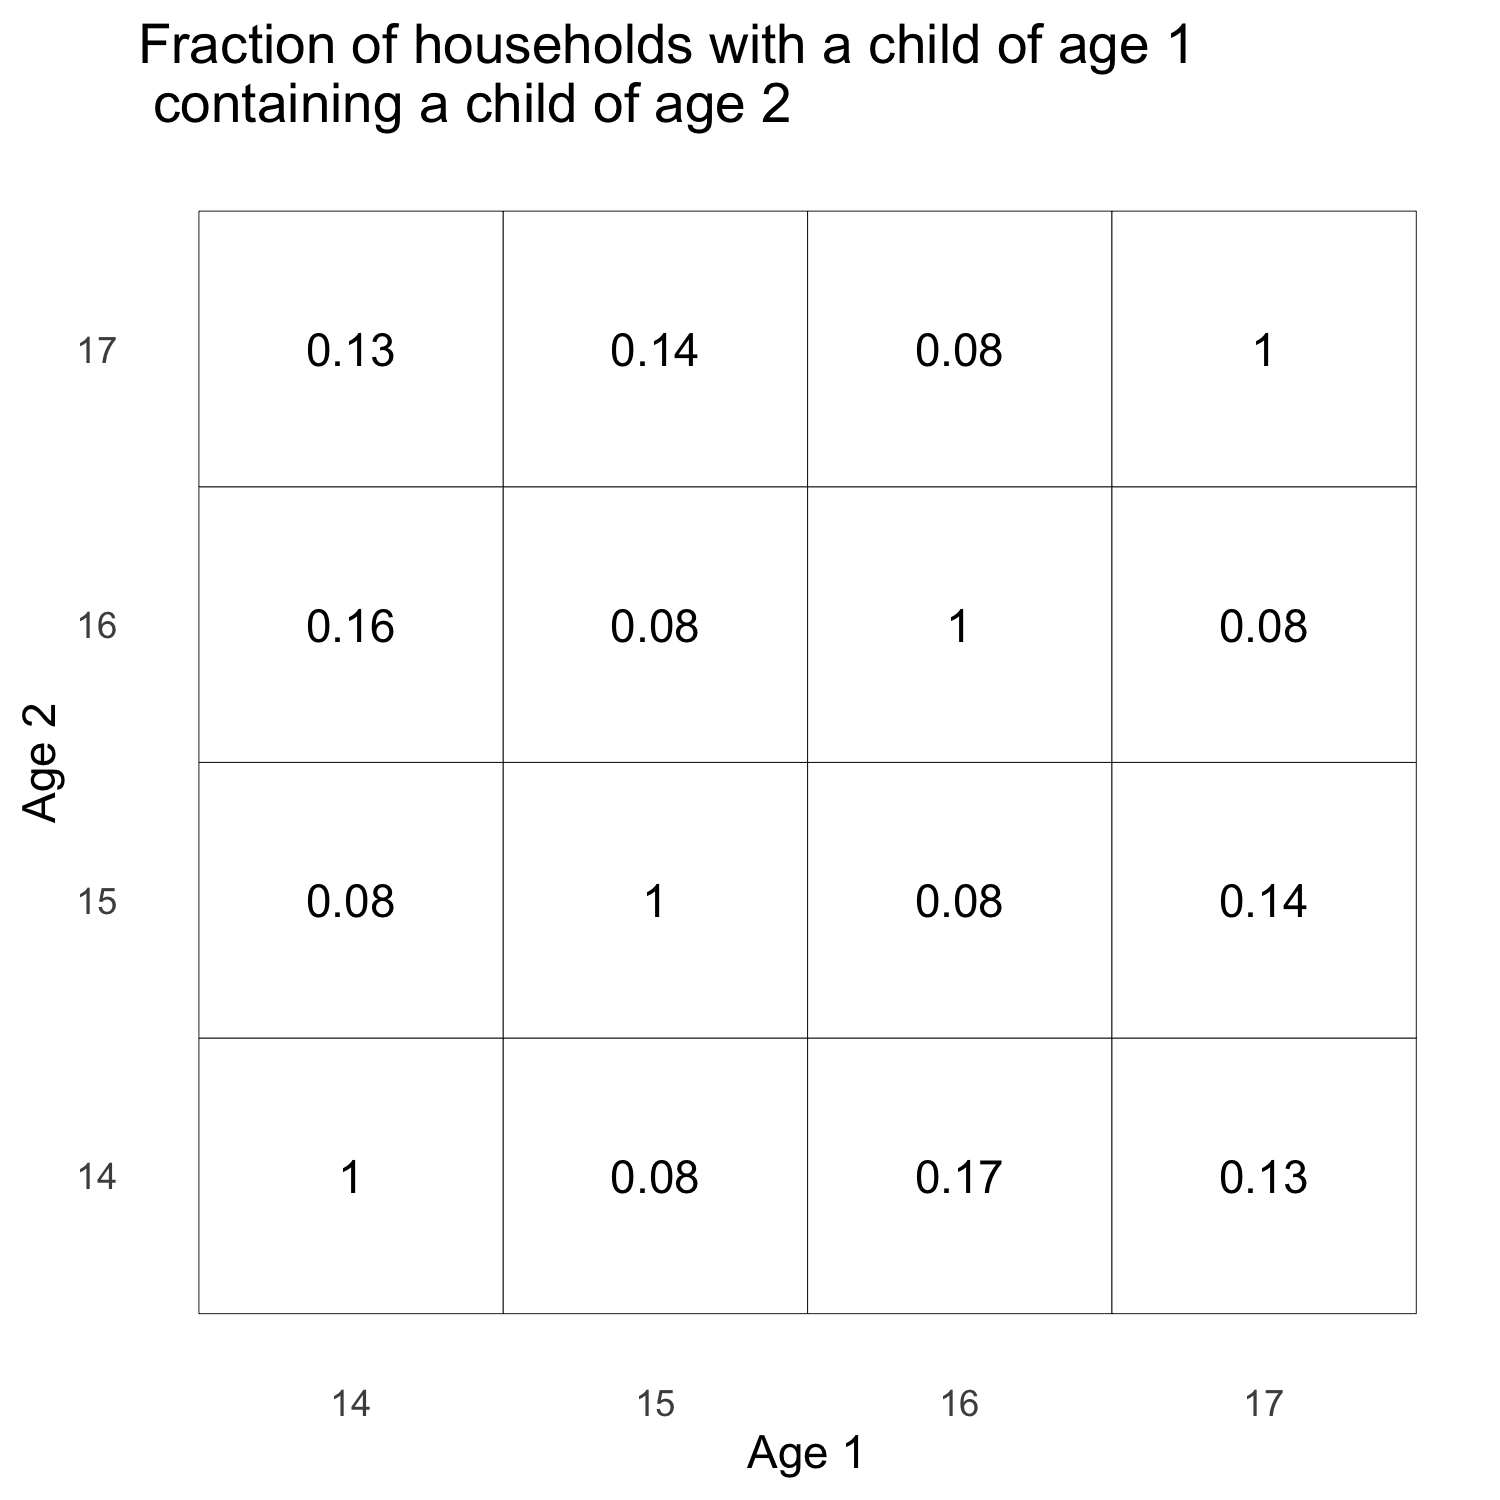
\includegraphics[width=40mm]{/Users/abilinski/Dropbox/Schools/Public code/0 - Synthetic Populations/2 - Output/sibling_heatmap_Texas_HS.png} 
    \end{tabular}

\clearpage

\hypertarget{references}{%
\section*{References}\label{references}}
\addcontentsline{toc}{section}{References}

\hypertarget{refs}{}
\leavevmode\hypertarget{ref-wheaton_us_2014}{}%
Wheaton, W. D. 2014. ``U.S. Synthetic Population 2010 Version 1.0 Quick
Start Guide, RTI International.''

\end{document}
